\scanpage{15}
\mspage{5}

imply
\[
\text{b')}\quad\varphi_!(F\times G)\longrightarrow\varphi_!(F)\times\varphi_!(G)\quad\text{epimorphism}
\qquad\forall F,G\text{ in }\operatorname{Ob}\widehat A
\]
\[
\text{c')}\quad\varphi_!(G\times_F H)\longrightarrow
\varphi_!(G)\times_{\varphi_!(F)}\varphi_!(H)\quad\text{epimorphism}
\]
$\forall$ diagram
\diagram{\begin{tikzcd}[ampersand replacement=\&,column sep=small,row sep=small]
G\arrow[dr]\&\&H\arrow[dl]\\
\&F\&
\end{tikzcd}}
in $\widehat A$.

and hence, more generally, the single equivalent form of Hypotheses 1, 2, 2' :

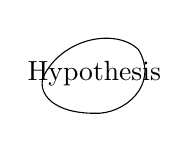
\begin{tikzpicture}[baseline=(n.base)]\node[inner sep=0pt] (n) at (0,0) {Hypothesis};\draw (-.65,-.05)..controls(-.4,.46)and(.28,.57)..(.56,.3)..controls(.83,-.15)and(.38,-.53)..(0,-.51)..controls(-.51,-.51)and(-.72,-.27)..(-.65,-.05);\end{tikzpicture}
For every finite diagram $(F_i)_{i\in I}$ in $\widehat A$, the canonical arrow
\[
\varphi_!\left(\varprojlim_I F_i\right)\longrightarrow\varprojlim_I\varphi_!(F_i)
\]
is an epimorphism.

(It suffices moreover to postulate it when the $F_i$ are in $A$, and in the three particular cases $I=\bullet$, $\bullet\ \bullet$,
\diagram{\begin{tikzcd}[ampersand replacement=\&,column sep=tiny,row sep=tiny]
\bullet\arrow[dr]\&\&\bullet\arrow[dl]\\
\&\bullet\&
\end{tikzcd}}, corresponding to the axioms Hypothesis 1, Hypothesis 2, Hypothesis $2'$.)

But can this hypothesis be satisfied, without $\varphi_!$ being $=$ left exac\textsuperscript{t} ?

\margin{14}
